\section*{Serverless Architecture \& Performance Evaluation}

% % \todo{Jerad will work on it}\\
% Nowadays, Linux workloads can be categorized into three parts: containers, virtualization, and language VM isolation.

% Here is the general view of serverless architecture shown in \reffig{fig:arc_serverless}. When a invoke occurs, frontend Invoke REST API gets the request and check for authorization and load the function metadata. 

% \todo{Jerad: please complete the rest of the part: check section: 4.1.1}

% \todolink{https://assets.amazon.science/96/c6/302e527240a3b1f86c86c3e8fc3d/firecracker-lightweight-virtualization-for-serverless-applications.pdf}

% \begin{figure}[!ht]
% 	\centering
% 	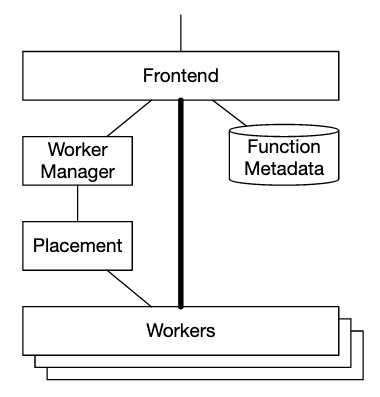
\includegraphics[width=0.5\textwidth]{images/serverless_architecture.png}
% 	\caption{Serverless Worker-Manager architecture \cite{firecracker}}
% 	\centering
% 	\label{fig:arc_serverless}
% \end{figure}


\label{sec:solution}
\subsection*{SCAR: Serverless Computing for Container-based Architectures}
This paper proposed a methodology to create Serverless Container-aware ARchitectures (SCAR) \cite{PEREZ201850} to solve the installation and deployment of external libraries that are not predefined. The SCAR can be used to serve event-driven and highly-parallel serverless applications that run on customized runtime environments defined as Docker images on top of AWS Lambda. \reffig{fig:scar_architecture} shows the architecture of SCAR. SCAR enables users to assign Lambda functions. When an invocation occurs, a container from the Docker image, which is stored in a Docker hub, will be executed. The architecture has two sections: SCAR client and SCAR server. SCAR Client is a python script to validate input, create the deployment including udocker, create the Lambda function with SCAR supervisor, manage the configuration to trigger events from S3~\cite{s3} to Lambda. SCAR server represents the Lambda function's code (Python 3.6) and retrieves the Docker image using udocker from Docker hub. First, the user selects a Docker image available in Docker Hub and generates the Lambda with the user's configuration. The user can directly invoke the Lambda function where the SCAR supervisor is triggered, which is ended up executing a container out of a Docker image and optionally run a user-defined shell script. Data staging from and to S3 is automatically managed by the SCAR supervisor and diverted the logs into CloudWatch.
\begin{figure}[!t]
	\centering
	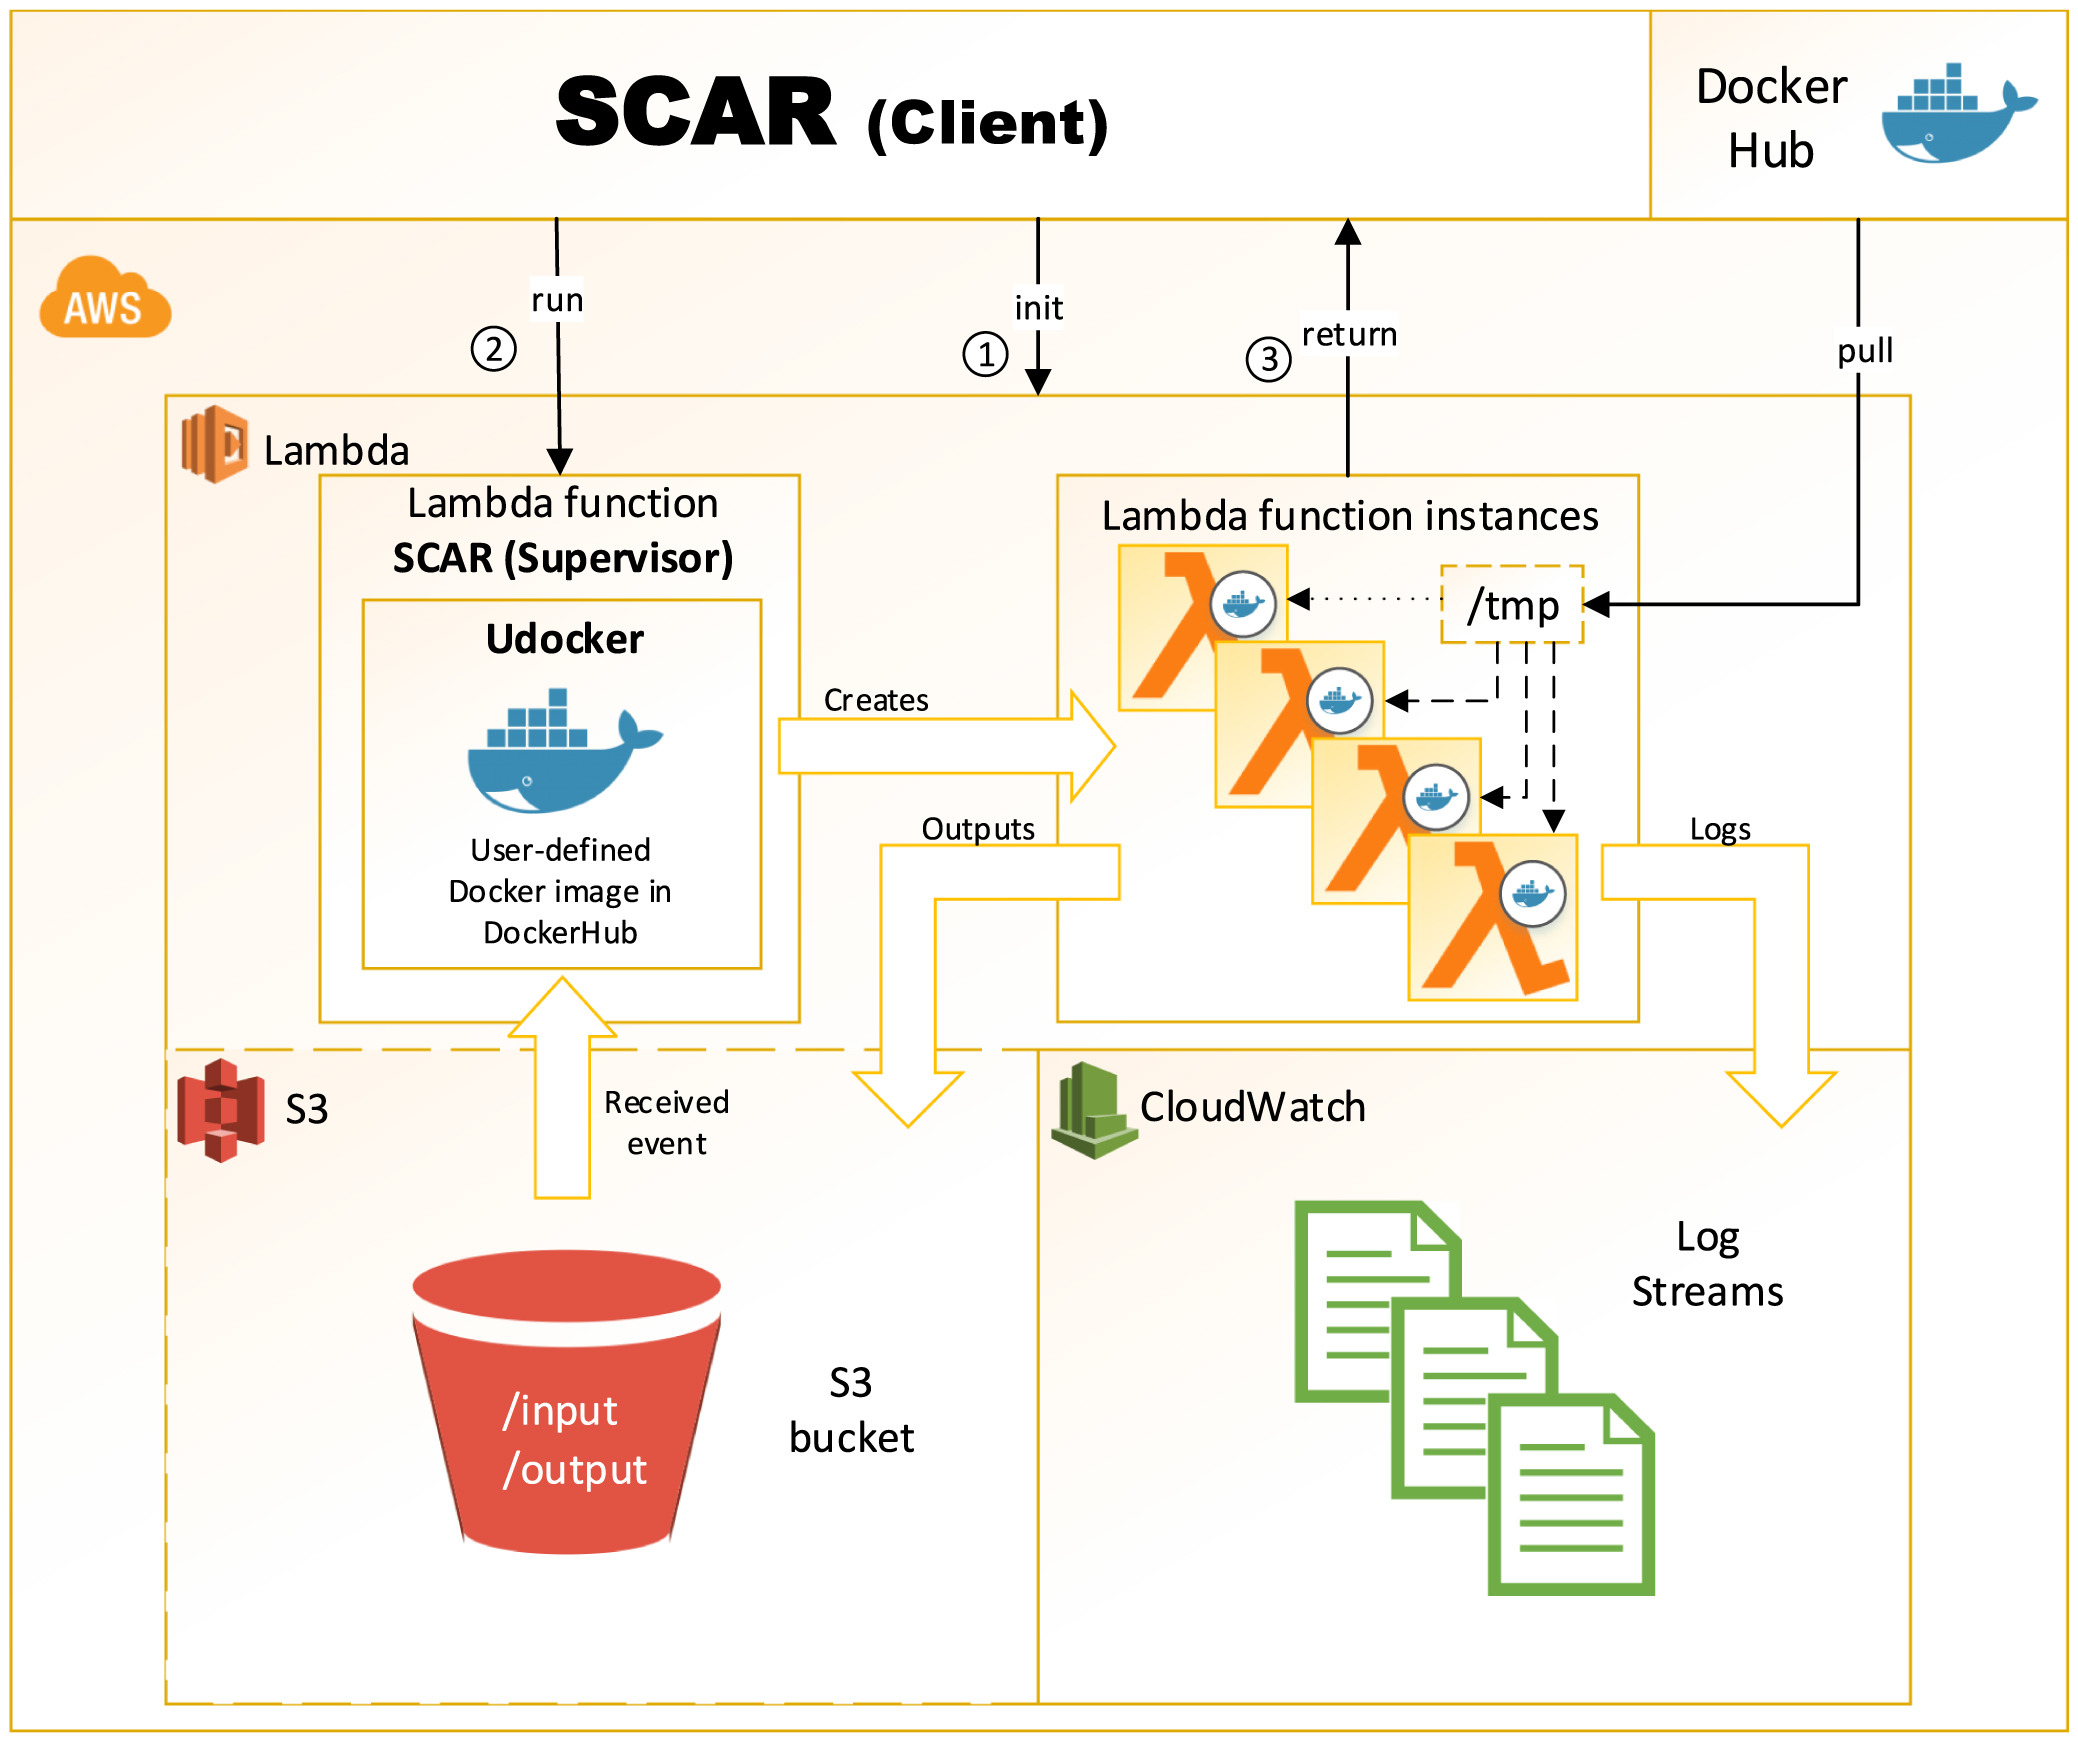
\includegraphics[width=0.7\textwidth]{images/scar_architecture.jpg}
	\caption{SCAR Architecture \cite{PEREZ201850}}
	\centering
	\label{fig:scar_architecture}
\end{figure}

\begin{figure*}[!b]
\centering % <-- added
\begin{subfigure}{0.32\textwidth}
  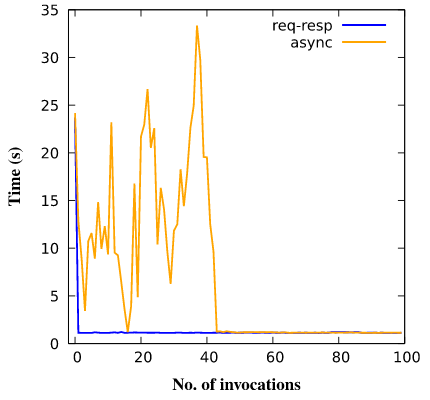
\includegraphics[width=\linewidth]{images/scar-1.png}
  \caption{Average execution time(in seconds) for each invocation type \cite{PEREZ201850}}
  \label{fig:scar1}
\end{subfigure} \hfil% <-- added
\begin{subfigure}{0.33\textwidth}
  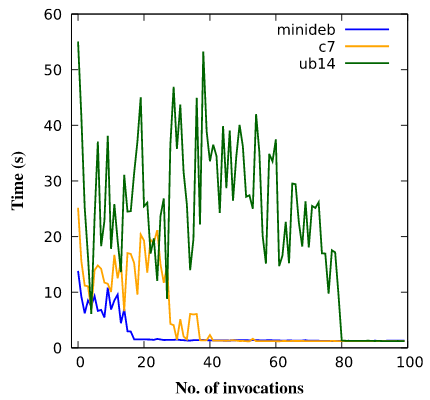
\includegraphics[width=\linewidth]{images/scar-3.png}
  \caption{Average execution time (in seconds) for different container sizes (all synchronous) \cite{PEREZ201850}}
  \label{fig:scar3}
\end{subfigure} \hfil% <-- added
\begin{subfigure}{0.33\textwidth}
  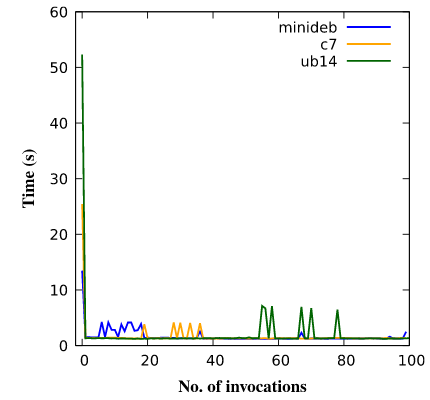
\includegraphics[width=\linewidth]{images/scar-4.png}
  \caption{Average execution time (in seconds) for different container sizes (First invocation req-res and subsequent are asynchronous) \cite{PEREZ201850}}
  \label{fig:scar4}
\end{subfigure} \hfil% <-- added
\caption{SCAR Performance}
\label{fig:scar_performance}
\end{figure*}
% \begin{itemize}
%     \item SCAR Client: It is a python script to validate input, create the deployment including udocker, create the Lambda function with SCAR supervisor, manage the configuration to trigger events from S3 to Lambda.
%     \item SCAR Server: 
% \end{itemize}

\reffig{fig:scar_performance} shows the performance of SCAR where \reffig{fig:scar1} refers the average execution time for each invocation type. The \textit{req-resp} means the request-response invocation type, and the \textit{async} means asynchronous invocation type. Here, the \textit{req-resp} initially takes 25s to download the container image from the docker hub, and after that next invocations execute instantly. On the other hand, the \textit{async} shows unpredictable behavior for the first 40 invocations. As SCAR caches the file system in the Lambda invocation's temporary space, it is normal to run instantly after the first invocation for the req-resp. However, the \textit{async} shows erratic behavior because all the invocations execute simultaneously. The invoked function cannot find the container cache and download from the docker hub and create a container. \reffig{fig:scar3} shows the average execution time for different container sizes for all asynchronous invocations. The authors want to show how the container size affects the caching performance for all asynchronous invocations. The \textit{minideb} means docker image \textit{bitnami/minideb} (size: 22MB), the \textit{c7} means \textit{centos:7} (size: 70MB) and the \textit{ub14} means \textit{grycap/jenkins:ubuntu14.04-python} (size: 153MB). The graph points out that the increasing container size takes higher time and higher invocations to store the temporary disk space's cache. \reffig{fig:scar4} shows the SCAR's idea to use first req-resp invocation and then asynchronous invocations. As a result, the unpredictable behavior of caching has gone and reduces execution time and invocations to store the container cache.

\todo{needs to add\reffig{fig:scar3} shows the average execution time for different container sizes for all asynchronous invocations. The authors want to show how the container size affects the caching performance for all asynchronous invocations. The minideb means docker image bitnami/minideb (size: 22MB), the c7 means centos:7 (size: 70MB) and the ub14 means grycap/jenkins:ubuntu14.04-python (size: 153MB). The graph points out that the increasing container size takes higher time and higher invocations to store the temporary disk space's cache.limitations}

\subsection*{Firecracker: Lightweight Virtualization for Serverless}
\todo{Jerad please complete it, same paper}

\todolink{https://assets.amazon.science/96/c6/302e527240a3b1f86c86c3e8fc3d/firecracker-lightweight-virtualization-for-serverless-applications.pdf}


\begin{figure}[!ht]
	\centering
	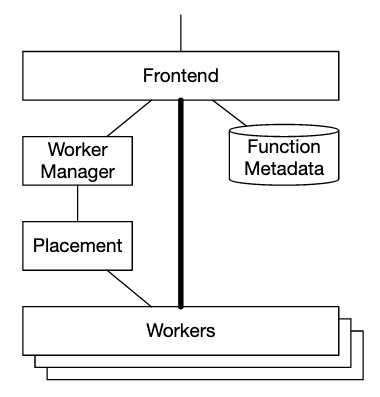
\includegraphics[width=0.35\textwidth]{images/serverless_architecture.png}
	\caption{Serverless Worker-Manager architecture \cite{firecracker}}
	\centering
	\label{fig:arc_serverless}
\end{figure}

\begin{figure*}[!t]
\centering % <-- added
\begin{subfigure}{0.35\textwidth}
  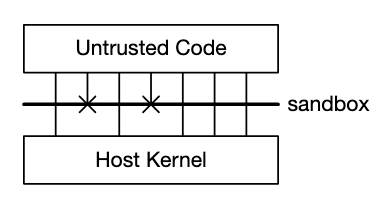
\includegraphics[width=\linewidth]{images/container_architecture.png}
  \caption{Container based Serverless architecture \cite{firecracker}}
  \label{fig:container_serverless}
\end{subfigure} \hfil% <-- added
\begin{subfigure}{0.35\textwidth}
  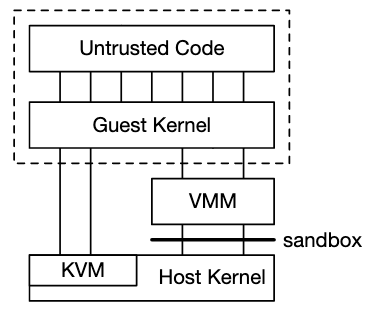
\includegraphics[width=\linewidth]{images/VM_architecture.png}
  \caption{VM based Serverless Architecture \cite{firecracker}}
  \label{fig:human_memory}
\end{subfigure} \hfil% <-- added

\caption{Serverless Architecture}
\label{fig:memory}
\end{figure*}

\subsection*{Lightweight Serverless Computing via Unikernel}
The startup delays of VMs or containers create a higher response latency to users and performance overhead. This paper introduces UaaF (Unikernel-as-a-Function) to provide a lightweight approach to serverless computing that offers a low startup latency to execute functions and a communication model for better inter-functions interactions \cite{tan2020unikernel}. The existing serverless frameworks install all the libraries by an application at startup in every sandbox. As a result, the application finds a high-level redundancy in the memory footprint and high latency in loading libraries. Around 2ms-800ms is needed to load the runtime library when a lambda invocation occurs for the first time, and 80\% of the startup latency is the library installation time \cite{verma2015google}. To avoid a cold start, the authors abstract fine-grained functions from codes and use these shareable libraries in different unikernels and use a special unikernel named ``session'' as a proxy of a serverless application. It holds the sequence of library function invocations and represents the serverless application in the task scheduler. As a result, a session can be executed more quickly. Moreover, UaaF installs separate stacks for different sessions within the virtual address space; therefore, the only copy of library functions need to be stored in the memory that decreases memory repetition across the serverless application shown in \reffig{fig:uaaf_abstraction}.
\begin{figure*}[!t]
\centering % <-- added

\begin{subfigure}{0.56\textwidth}
  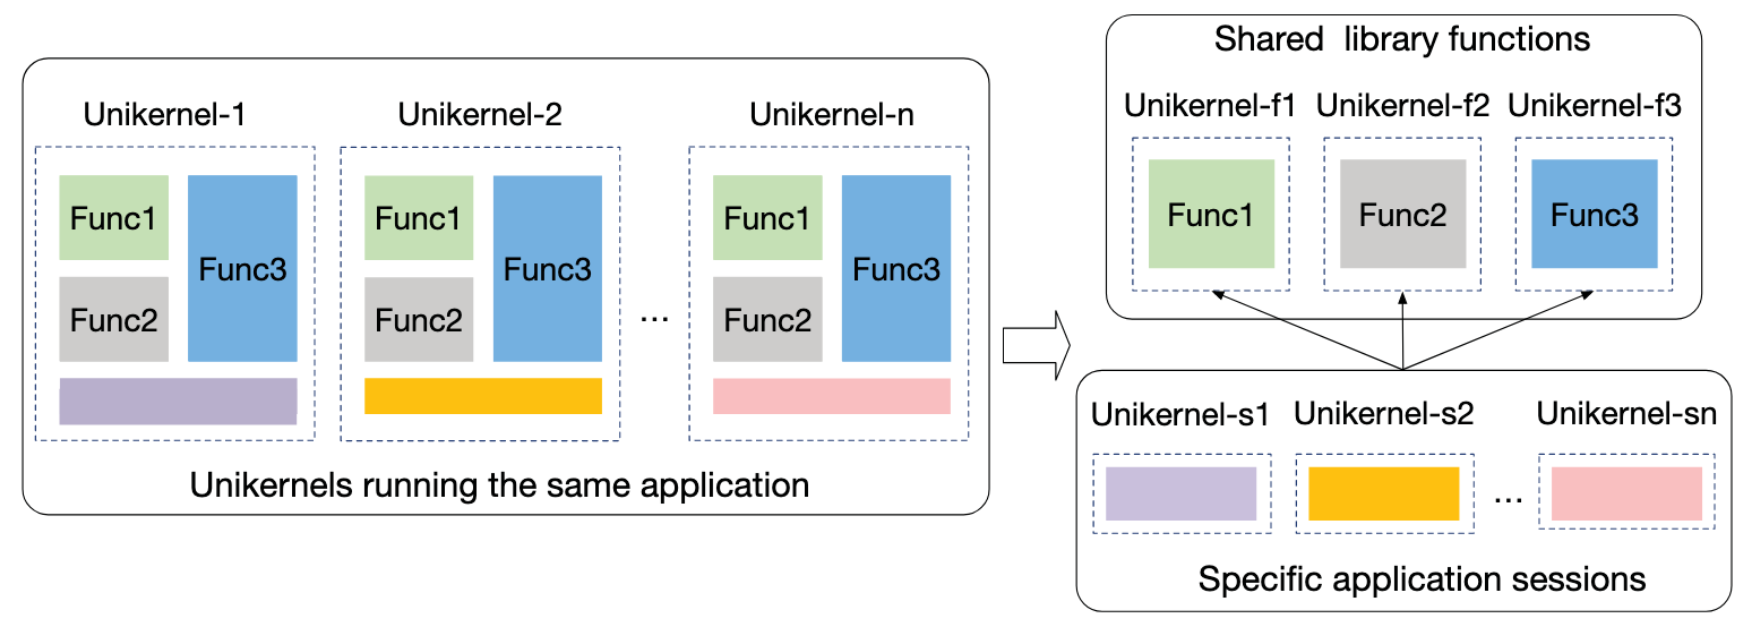
\includegraphics[width=\linewidth]{images/uaaf_abstraction.png}
  \caption{Functions are abstracted form applications and shared by multiple tasks in UaaF}
  \label{fig:uaaf_abstraction}
\end{subfigure} \hfil% <-- added
\begin{subfigure}{0.42\textwidth}
  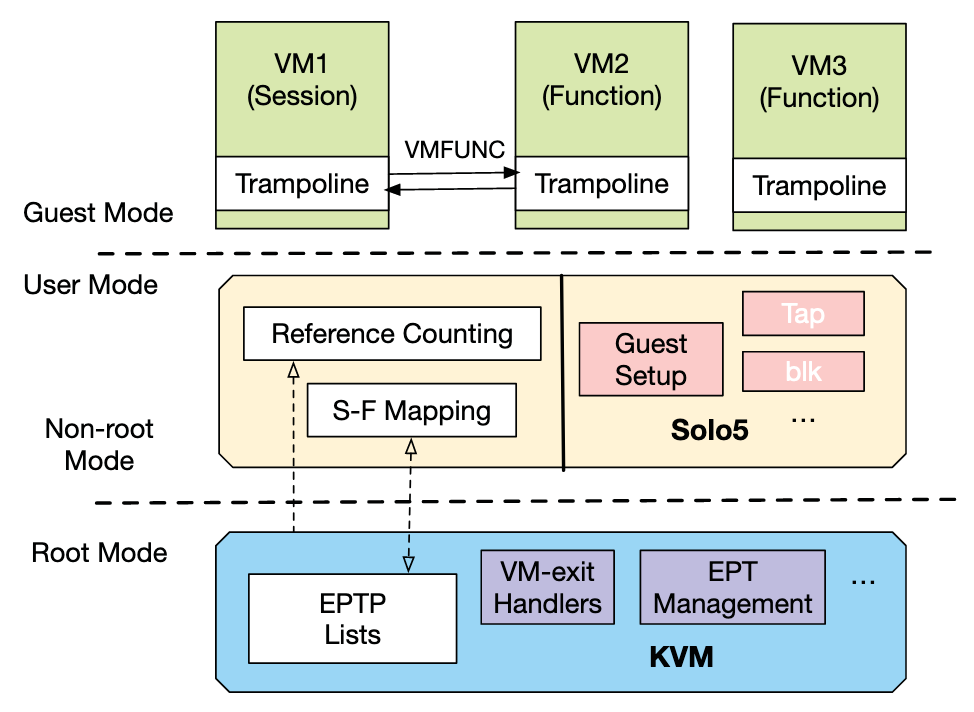
\includegraphics[width=\linewidth]{images/uaaf_architecture.png}
  \caption{The architecture of UaaF}
  \label{fig:uaaf_architecture}
\end{subfigure} \hfil% <-- added
\caption{Unikernel-as-a-Function \cite{tan2020unikernel}}
\label{fig:uaaf}
\end{figure*}
Here is the architecture of UaaF shown in \reffig{fig:uaaf_architecture}. The white modules are proposed by the authors and rests exist in original KVM \cite{kvm} and Solo5 \cite{solo5}. An EPTP (Extend Page Table Pointer) list is a special memory page in the KVM kernel space that has at most 512 EPTP entries pointing to the EPT of other unikernels. The list stores EPT entries used by the VMFUNC instructions. Each unikernel has a trampoline that is used to handle the remote calls between unikernels. UaaF has two modules in user mode. The session-function (S-F) mapping module maintains the mappings between the session ID and the EPTP ID in a table. The reference counting module stores the number of references to each of the functions. The functions that are not referenced, are destroyed by the UaaF.
\begin{figure*}[!b]
\centering % <-- added

\begin{subfigure}{0.34\textwidth}
  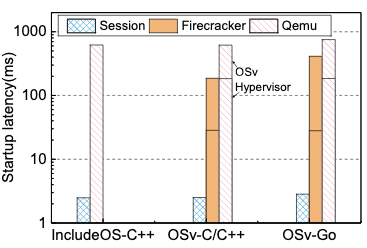
\includegraphics[width=\linewidth]{images/uaaf_start_lat.png}
  \caption{The startup latency of sessions and functions in UaaF}
  \label{fig:uaaf_start_lat}
\end{subfigure} \hfil% <-- added
\begin{subfigure}{0.31\textwidth}
  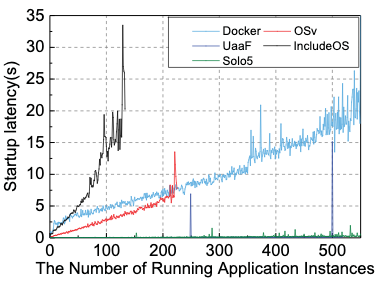
\includegraphics[width=\linewidth]{images/uaaf_start_lat_multiple.png}
  \caption{The startup latency varies with the number of application instances}
  \label{fig:uaaf_startvsmulti}
\end{subfigure} \hfil% <-- added
\begin{subfigure}{0.33\textwidth}
  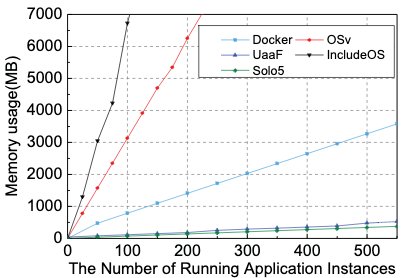
\includegraphics[width=\linewidth]{images/uaaf_multiple_memory.png}
  \caption{The memory usage of differentfunctions and containers}
  \label{fig:uaaf_memoryvsmultiple}
\end{subfigure} \hfil% <-- added
\caption{The performance of UaaF \cite{tan2020unikernel}}
\label{fig:uaaf_performance}
\end{figure*}
\reffig{fig:uaaf_performance} shows the performance of UaaF. \reffig{fig:uaaf_start_lat} shows the startup latency of sessions and functions in UaaF. As UaaF preloaded the functions in memory, the front-end sessions can be started instantly, and UaaF can also limit the application's startup latency below 3ms, which is faster than Firecracker and other traditional unikernels. \reffig{fig:uaaf_startvsmulti} shows the startup latency varies with the number of application instances. As each instance consisted of one session function, and multiple library functions were shared among all instances in UaaF, it can scale large instances similar to Solo5. \reffig{fig:uaaf_memoryvsmultiple} describes the memory usage of different-functions and containers. As we know, IncludeOS, Docker and OSv do not support instances to share execution environments. So, their memory increases linearly with the increasing number of instances. On the other hand, UaaF provides similar memory usage to Solo5 since all library functions were shared.

\todo{Saidur: needs to add limitations}


% \begin{figure}[!ht]
% 	\centering
% 	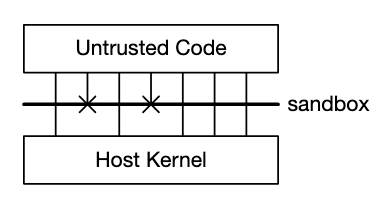
\includegraphics[width=0.5\textwidth]{images/container_architecture.png}
% 	\caption{}
% 	\centering
% 	\label{fig:container_serverless}
% \end{figure}

% \subsection*{VM based serverless}

% \begin{figure}[!ht]
% 	\centering
% 	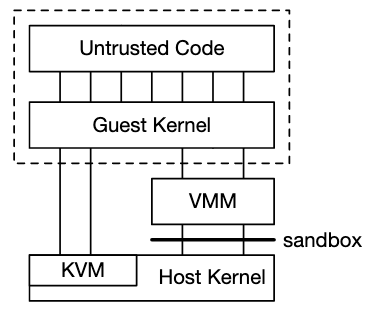
\includegraphics[width=0.5\textwidth]{images/VM_architecture.png}
% 	\caption{VM based Serverless Architecture \cite{firecracker}}
% 	\centering
% 	\label{fig:vm_serverless}
% \end{figure}


